\documentclass[lang=en,11pt]{elegantbook}

\title{Suncoast's Jumpstart Program}
\subtitle{Solution Manual}

\author{Cole Ellis, Jonathan Hartman, \& Joshua Kuffour}
\institute{Suncoast High School}
\date{1 June 2020}
\version{1.00}

\extrainfo{We are the World.}

\logo{suncoastShield.png}
\cover{FrontCover.jpg}

\pagecolor{white}

\begin{document}

\maketitle

\frontmatter
\tableofcontents

\mainmatter

%%%%%%%%%%%%%%%%%%%%%%%%%%%%%%%%%%%%%%%% CHAPTER 1 %%%%%%%%%%%%%%%%%%%%%%%%%%%%%%%%%%%%%%%

\chapter{Introduction}
This book contains the solutions to every review set and challenge set in the Suncoast's Jumpstart Program \textit{Curriculum Companion}.

In most problems, the final answer is contained in a box, $\boxed{\text{like this}}$.  Each solution is ended with a "Q.E.D." box ($\Box$).  Even if you got a problem right, we recommend reading the solution we provide; there is a chance you may find a new way of solving a problem!  

If you believe to have found in error in one of our solutions, email Mr. Ellis  \href{mailto:educationelite1@gmail.com}{here} with your detailed solution.
%%%%%%%%%%%%%%%%%%%%%%%%%%%%%% CHAPTER 2 %%%%%%%%%%%%%%%%%%%%%%%%%%%%%%%%%%%%%%%%%%%%%
\chapter{Function Basics}
\noindent \textbf{Review . 1}

(a) The lower bound is $7$ (inclusive) and the upper bound is $+\infty$ (exclusive).  This makes the interval notation $\boxed{[7,\infty)}$. $\Box$

(b) The lower bound is $5$ (inclusive) and the upper bound is $25$ (inclusive).  This makes the interval notation $\boxed{\left[5,25\right]}$. $\Box$

(c) The first interval is $\left[12,\dfrac{25}{2}\right]$.  The second interval is $[5]$.  Combining the two gives the final interval: $\boxed{[5] \cup \left[12,\dfrac{25}{2}\right]}$. $\Box$

(d) The first interval is $(-\infty,7]$.  The second interval is $[9]$.  The third interval is $[12,\infty)$.  Combining gives the interval $\boxed{(-\infty,7] \cup [9] \cup [12,\infty)}$. $\Box$\vspace{3mm}

\noindent \textbf{Review . 2}

(a) Since this is a polynomial, the domain is $\mathbb{R}$.  To find the range, we quickly see that $f(x)$ goes up infinitely but has a minimum value.  The minimum value comes by minimizing the $x^2$ term, which is when $x=0$.  At $x=0$, $f(0)=2(0)^2+3=3$.  This makes the range $[3,\infty)$.  So, our final answer is $\boxed{\begin{matrix} x\in\mathbb{R} \\ y\in[3,\infty) \end{matrix}}$. $\Box$

(b) We know that square roots must always be positive.  So, we must solve $12-(x-3)^2 \geq 0$.  Solving this with square roots, we get \begin{align*}
    12-(x-3)^2 &\geq 0 \\ 
    12 &\geq (x-3)^2 \\
    x-3 \geq -\sqrt{12} \hspace{0.15in} & \hspace{0.15in} (x-3) \leq \sqrt{12} \\
    x \geq 3-2\sqrt{3} \hspace{0.15in} & \hspace{0.15in} x \leq 3+2\sqrt{3}
\end{align*}

This gives the domain as $-9 \leq x \leq 15$.  Now we must determine the range in this interval.  We know that quadratics attain a maximum or minimum value at their vertex depending on their orientation.  Since this is an inverted quadratic, it attains a maximum at the vertex.  The maximum is attained when $(x-3)^2=0$, meaning $x=3$.  Plugging this in, we get $$f(3)=3+\sqrt{12}=3+2\sqrt{3}.$$  The minimums are at the endpoints of the domain, which is when the square root is minimized.  This gives $$f\left(3-2\sqrt{3}\right)=3+\sqrt{0}=3.$$  This gives the range of $3\leq y\leq 3+2\sqrt{3}$.  Thus, the final answer is $\boxed{\begin{matrix} x\in\left[3-2\sqrt{3},3+2\sqrt{3}\right] \\ y\in\left[3,3+2\sqrt{3}\right] \end{matrix}}$. $\Box$

(c) For this, we know that the denominator can't equal zero nor can the square root be negative.  Due to the square root, $x-1\geq 0$, so $x\geq 1$.  Due to the denominator, $2+\sqrt{x-1}\neq 0 \implies \sqrt{x-1}\neq -2$.  This is never true, so we ignore it.  So, our domain is $x\geq 1$.  

To find the range, we see that the lower bound of the function is $0$ by noting that as $x\to \infty$, $f(x) \to 0$.  However, $f(x)$ never reaches $0$, so it will be a exclusive bound.  To find the upper bound, we simply note that $f(x)$ is decreasing over the entire interval, so the lower bound of the domain gives us the value we need.  $f(1)=\dfrac{1}{2+\sqrt{0}}=\dfrac{1}{2}$.  This means that the range is $0 < f(x) \leq \dfrac{1}{2}$.  

So, our final answer is $\boxed{\begin{matrix} x\in[1,\infty) \\ y\in\left(0,\dfrac{1}{2}\right] \end{matrix}}$. $\Box$

(d) Since the denominator can't equal zero, we get the domain to be $x\neq \dfrac{1}{3}$.  To find the range, we must take the inverse.  Below is this process.\begin{align*}
    f(x)&=\dfrac{2x-3}{3x-1} \\
    x&=\dfrac{2f^{-1}(x)-3}{3f^{-1}(x)-1} \\
    3xf^{-1}(x)-x &= 2f^{-1}(x)-3 \\
    (3x-2)f^{-1}(x)&=x-3 \\
    f^{-1}(x)&=\dfrac{x-3}{3x-2}
\end{align*}

The domain restriction of $f^{-1}(x)$ is $x\neq \dfrac{2}{3}$, so we know the range of $f(x)$ is $f(x)\neq \dfrac{2}{3}$.  So, our final answer is $\boxed{\begin{matrix} x\in\left(-\infty,\dfrac{1}{3}\right)\cup\left(\dfrac{1}{3},\infty\right) \\ y\in\left(-\infty,\dfrac{2}{3}\right)\cup\left(\dfrac{2}{3},\infty\right) \end{matrix}}$. $\Box$\vspace{3mm}

\noindent \textbf{Review . 3}

Let's determine the domain for both of them.  $f(x)$ is restricted since $x-3 \neq 0$ and $\dfrac{2x-1}{x-3} \geq 0$.  Due to the first restriction, $x\neq 3$.  Due to the second restriction, $x \geq 3$ or $x\leq \dfrac{1}{2}$.  (\textit{Make sure you see why!})  This gives the domain as $x\in\left(-\infty,\dfrac{1}{2}\right)\cup\left(3,\infty\right)$.

Now to work out the domain of $g(x)$.  We see that $x-3\neq 0$, $x-3 \geq 0$, and $2x-1\geq 0$.  This means that $x>3$ and $x\geq \dfrac{1}{2}$. Combining these, we get $(3,\infty)$. 

As we can see, $\boxed{f(x) \text{ and } g(x) \text{ have different domains}}$. $\Box$\vspace{3mm}

\noindent \textbf{Review . 4}

No!  $f(x)$ has a clear domain restriction at $x=1$ that $g(x)$ doesn't have.  Thus, $\boxed{f(x) \text{ and } g(x) \text{ are not the same}}$. $\Box$\vspace{3mm}

\noindent \textbf{Review . 5}

(a) We know that all polynomials pass the vertical line test. This means that it is a function.  Now we must determine if the inverse is a function.  There are two ways to consider this: graphically and algebraically.  Graphically, we know that parabolas have a "U"-shape, which fails the horizontal line test.  This means that $\boxed{f(x) \text{ is not one-to-one}}$.

Algebraically, we search for a value of $k$ such that $f(x)=k$ for more than one value of $x$.  So, we let $f(x)=k$ and solve for $x$. \begin{align*}
    2x^2-x-3&=k \\ 2x^2-x-(3+k)&=0 \\ x&=\dfrac{1\pm\sqrt{23-8k}}{4}
\end{align*}
If you don't understand what just happened here, we used the quadratic formula.  It is covered in section 5.8 of the \textit{Curriculum Companion}.  All we need to do is make sure that $x$ is defined.  Thus, $23-8k>0$, meaning $k>\dfrac{23}{8}$.  So, for any value of $k>\dfrac{23}{8}$, $f(x)$ has two values of $x$ for the same value of $k$.  This fails the horizontal line test and thus is $\boxed{\text{not one-to-one}}$.$\Box$

\begin{remark}
Note that we used $>$ rather than $\geq$.  This is because if the square root equals zero, it still yields one value (because of the $\pm$).
\end{remark}

(b) We will attempt to solve this problem algebraically.  We know that rational equations are indeed functions over their domain.  We need to make sure that the inverse is also a function.  We look for $k$ such that $f(x)=k$ for more than one $x$.  We let $f(x)=k$ and solve for $x$: $$\dfrac{1}{2x-1} = k \implies 1=2kx-k \implies \dfrac{1+k}{2k}=x.$$
This simply produces another rational function which we know is a function.  This means that there is no value of $x$ to produce more than one $k$, so $\boxed{f(x)\text{ is one-to-one}}$.

Alternatively, we could've found a solution by taking the inverse of $f(x)$.  We get the inverse to be \begin{align*}
    f(x)&=\dfrac{1}{2x-1} \\ x&=\dfrac{1}{2f^{-1}(x)-1} \\ 2xf^{-1}(x)-x&=1 \\ f^{-1}(x)&=\dfrac{1-x}{2x}
\end{align*}
Note that this is the same function we had in the previous method!  We actually found the inverse in that process without even realizing it, which further proves our answer is right. $\Box$

(c) This is best considered graphically.  For every value on the circle except the maxima and minima for $x$ and $y$, a vertical or horizontal line can be used to touch more than one point.  This means that the equation given isn't a function, nor is its inverse, meaning that it's $\boxed{\text{not one-to-one}}$. $\Box$

(d) This problem looks difficult at first, but there's a trick to it.  Note that this function is simply the inverse of $y(x)=x^2-x-2$; we know this since the $x$'s and $y$'s are switched!  Since $y(x)$ fails the horizontal line test, this must mean that the equation given fails the vertical line test, making it not a function.  Thus, it is $\boxed{\text{not one-to-one}}$. $\Box$ \vspace{3mm}

\noindent \textbf{Problem . 6}

(a) If $f(x)=x^2$, the inverse must be $x=\left(f^{-1}(x)\right)^2$, which means $f^{-1}(x)=\sqrt{x}$.  However, we must note that $x\geq 0$ so that $f^{-1}(x)$ is defined.   So, the final answer is $\boxed{f^{-1}(x)=\sqrt{x}, \hspace{0.1in} x\geq 0}$.$\Box$

(b) Below is the process for finding $f^{-1}(x)$. \begin{align*}
    f(x)&=\dfrac{x-2}{x+2} \\ x&=\dfrac{f^{-1}(x)-2}{f^{-1}(x)+2} \\ xf^{-1}(x)+2x&=f^{-1}(x)-2 \\ (x-1)f^{-1}(x)=-2x-2 \\ f^{-1}(x)=\dfrac{-2(x+1)}{x-1}
\end{align*}
$f(x)$ had a domain restriction at $x=2$.  $f^{-1}(x)$ has a domain restriction at $x=1$.  So, our final answer must be $\boxed{f^{-1}(x)=\dfrac{-2(x+1)}{x-1}, \hspace{0.1in} x\neq 1,2}$. $\Box$

(c) If $f(x)=\dfrac{1}{x^4}$, this means that $x^4=\dfrac{1}{f(x)}$.  Switching $x$ and $f(x)$, we get $\left(f^{-1}(x)\right)^4=\dfrac{1}{x}$, or $f^{-1}(x)=\dfrac{1}{\sqrt[4]{x}}$.  We need to add the domain restriction that $x>0$ due to the denominator.  Thus, $\boxed{f^{-1}(x)=\dfrac{1}{\sqrt[4]{x}}, \hspace{0.1in} x>0}$. $\Box$

\noindent \textbf{Problem . 7}

(a) We know that the parent function of $f(x)$ is a parabola ("U") centered at $(0,0)$.  This is shifted one to the right.  When we graph $f(x)$ and the inverse, we also mark $y(x)=x$ to denote the line of reflection.
\begin{figure}[!ht]
    \centering
    \begin{tikzpicture}[xscale=0.25,yscale=0.25]
      \draw[<->] (-10,0) -- (10,0) node[right] {$x$};
      \draw[<->] (0,-10) -- (0,10) node[above] {$y(x)$};
      \draw[scale=1,domain=-2.7:3.7,smooth,variable=\x,black] plot ({\x},{\x*\x-\x}) node[right] {$f(x)$};
      \draw[scale=1,domain=-2.7:3.7,smooth,variable=\y,black] plot ({\y*\y-\y},{\y}) node[right] {$f^{-1}(x)$};
      \draw[scale=1,domain=-10:10,smooth,variable=\x,black,dashdotted] plot ({\x},{\x});
    \end{tikzpicture}   
\end{figure}

(b) The parent function of this is $f_0(x)=\sqrt{x}$, which is the upper-half of a sideways parabola centered at $(0,0)$.  The factor of $\sqrt{2}$ creates a vertical stretch.  Factoring the two, we get $f(x)=\sqrt{2\left(x-\dfrac{1}{2}\right)}$.  This means that $f_0(x)$ is shifted $\dfrac{1}{2}$ unit to the right.  Below is the graph of $f(x)$ and its inverse.

\begin{figure}[!ht]
    \centering
    \begin{tikzpicture}[xscale=0.25,yscale=0.25]
      \draw[<->] (-10,0) -- (10,0) node[right] {$x$};
      \draw[<->] (0,-10) -- (0,10) node[above] {$y(x)$};
      \draw[scale=1,domain=0:4.35,smooth,variable=\y,black] plot ({\y*\y/2+1/2},{\y}) node[right] {$f(x)$};
      \draw[scale=1,domain=0:4.35,smooth,variable=\x,black] plot ({\x},{\x*\x/2+1/2}) node[right] {$f^{-1}(x)$};
      \draw[scale=1,domain=-10:10,smooth,variable=\x,black,dashdotted] plot ({\x},{\x});
    \end{tikzpicture}   
\end{figure}

(c) The parent function is $f_0(x)=\dfrac{1}{x}$.  Factoring the $2$ from the denominator gives $f(x)=\dfrac{3}{2}\cdot \dfrac{1}{x+2}+1$. We see that the graph is shifted from the original center at $(0,0)$ to $(-2,1)$ and is scaled vertically by a factor of $\dfrac{3}{2}$.  Below is the graph of $f(x)$ and its inverse.

\begin{figure}[!ht]
    \centering
    \begin{tikzpicture}[xscale=0.25,yscale=0.25]
      \draw[<->] (-10,0) -- (10,0) node[right] {$x$};
      \draw[<->] (0,-10) -- (0,10) node[above] {$y(x)$};
      \draw[scale=1,samples=100,domain=-10:-2.06,variable=\x,black] plot ({\x},{1/(2*\x+4)-3});
      \draw[scale=1,samples=100,domain=-1.96:10,variable=\x,black] plot ({\x},{1/(2*\x+4)-3}) node[right] {$f(x)$};
      \draw[scale=1,samples=100,domain=-10:-2.06,variable=\y,black] plot ({1/(2*\y+4)-3},{\y}) node[left] {$f^{-1}(x)$};
      \draw[scale=1,samples=100,domain=-1.96:10,variable=\y,black] plot ({1/(2*\y+4)-3},{\y});
      \draw[scale=1,domain=-10:10,smooth,variable=\x,black,dashdotted] plot ({\x},{\x});
    \end{tikzpicture}   
\end{figure}

\noindent \textbf{Review . 8}

$$(f\circ g)(x)=\dfrac{3\left(\dfrac{2x}{x+3}\right)}{\left(\dfrac{2x}{x+3}\right)+2}=\dfrac{\dfrac{6x}{x+3}}{\dfrac{2x+2(x+3)}{x+3}}=\dfrac{6x}{4x+6}=\boxed{\dfrac{3x}{2x+3}}.$$$\Box$

\noindent \textbf{Review . 9}

Our goal is to find $g(2)$.  In terms of $a$, $b$, and $c$, this is $4a+2b-c$.  We know that $f(1)=g(1)+1$, which gives us $$a+b+c=a+b-c+1 \implies c=\dfrac{1}{2}.$$  We also know that $f(2)=4a+2b+c=2$, which means that $$4a+2b=2-c \implies 4a-2b=\dfrac{3}{2}.$$  Thus, we get $g(2)=\dfrac{3}{2}-\dfrac{1}{2}=\boxed{1}$. $\Box$  \vspace{3mm}

\noindent \textbf{Review . 10}

There isn't much new explanation to solving this one.  We graph $f(x)$ as the dotted graph and then each of the transformations.
\begin{figure}[!ht]
    \centering
    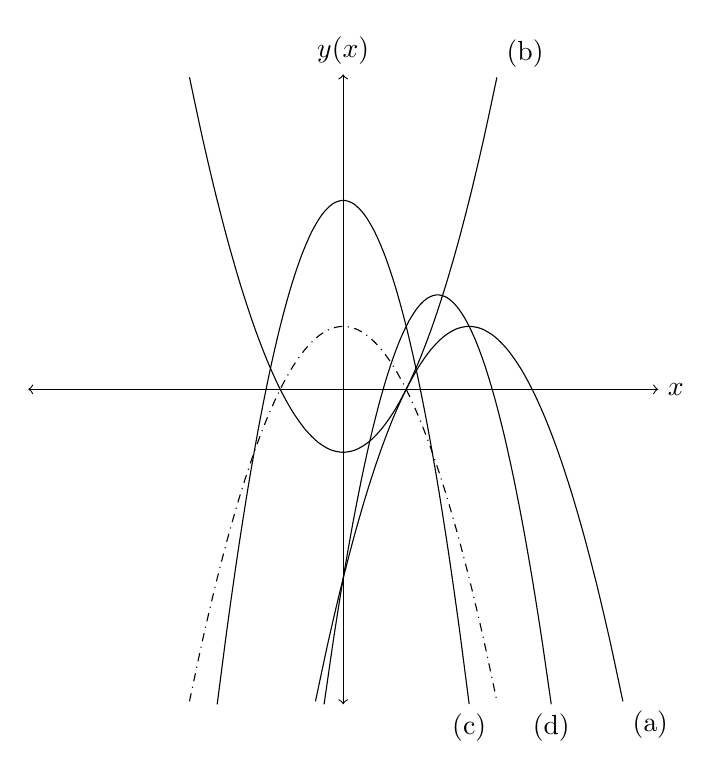
\begin{tikzpicture}[xscale=0.8,yscale=0.8]
      \draw[<->] (-5,0) -- (5,0) node[right] {$x$};
      \draw[<->] (0,-5) -- (0,5) node[above] {$y(x)$};
      \draw[scale=1,domain=-2.44:2.44,smooth,variable=\x,black,dashdotted] plot ({\x},{1-\x*\x});
      \draw[scale=1,domain=-0.44:4.44,smooth,variable=\x,black] plot ({\x},{-3-\x*\x+4*\x}) node[below right] {(a)};
      \draw[scale=1,domain=-2.44:2.44,smooth,variable=\x,black] plot ({\x},{-1+\x*\x}) node[above right] {(b)};
      \draw[scale=1,domain=-2:2,smooth,variable=\x,black] plot ({\x},{3-2*\x*\x}) node[below] {(c)};
      \draw[scale=1,domain=-0.303:3.303,smooth,variable=\x,black] plot ({\x},{-2*\x*\x+6*\x-3}) node[below] {(d)};
    \end{tikzpicture}   
\end{figure} 

If you want to find the actual equation (in standard form) here is the work: \begin{align*}
    f(x-2)&=1-(x-2)^2=1-(x^2-4x+3)=-x^2+4x-3 \\
    -f(x)&=-(1-x^2)=x^2-1 \\
    2f(x)-1&=2(1-x^2)+1=2-2x^2+1=-2x^2+3 \\
    \dfrac{1}{2}f(2x-3)+1&=\dfrac{1}{2}\left(1-(2x-3)^2\right)+1=\dfrac{1}{2}\left(-4x^2+12x-8\right)+1=-2x^2+6x-3
\end{align*}$\Box$

\noindent \textbf{Review . 11}

Our goal is to find a counterexample to this statement; if we cannot find one, we know that it must be true.  The only way for this statement to not be true is if $f(x)$ and $g(x)$ have the same domain and $(f\circ f)(x)$ and $(f\circ g)(x)$ to have the same domain.  The easiest way to accomplish this is to let $g(x)=x$.  That way, all we need to do is find $f(x)$ such that $(f\circ f)(x)=f(x)$.  Taking the inverse, we get $f(x)=f^{-1}\left(f(x)\right)$.  By definition, that means that $f(x)=x$.  However, there's another solution to this.  If we say $f(x)=|x|$, this only changes the range and not the function.  And $|(|x|)|=|x|$, so the statement holds.  This means that if $f(x)=|x|$ and $g(x)=x$, $(f\circ f)(x)=(f\circ g)(x)$, but $f(x)\neq g(x)$.  Thus, the statement is $\boxed{\text{false}}$. $\Box$ \vspace{3mm}

\noident \textbf{Review . 12}

All you need to do is take any negative $y$-value and reflect it over the $y$-axis. $\Box$

\noindent \textbf{Review . 13}

Using the property that the domain and range switch when we take the inverse, we know that we need to let $f(x)=4$ to find the answer.  Below is the work to solve for $x$: \begin{align*}
    \dfrac{2x-3}{3x-1}&=4 \\ 2x-3 &= 12x-4 \\ 1&=10x \\ \boxed{x=\dfrac{1}{10}}.
\end{align*} $\Box$

\noindent \textbf{Review . 14}

To graph each section, consider the parent functions and the corresponding transformations.  The first two bounds don't have any transformations, but the third is shifted one unit upward.  Below is the graph.
\begin{figure}[!ht]
    \centering
    \begin{tikzpicture}[xscale=0.25,yscale=0.25]
      \draw[<->] (-10,0) -- (10,0) node[right] {$x$};
      \draw[<->] (0,-10) -- (0,10) node[above] {$y(x)$};
      \draw[scale=1,samples=100,domain=-1.58:0,variable=\x,black] plot({\x},{\x*\x*\x*\x*\x});
      \draw[scale=1,samples=100,domain=5:10,variable=\x,black] plot({\x},{1/2});
      \draw[scale=1,samples=100,domain=0.33:5,variable=\x,black] plot({\x},{1/(\x*\x)+1});
      \filldraw (0,0) circle[radius=7pt];
      \filldraw (5,0.5) circle[radius=7pt];
      \draw (5,1) circle[radius=7pt];
    \end{tikzpicture}   
\end{figure} $\Box$

\noindent \textbf{Review . 15}

$$f(x) \cdot f(-x) =\left(\dfrac{2x-3}{3x-1}\right)\left(\dfrac{-2x-3}{-3x-1}\right)=\dfrac{-4x^2+9}{-9x^2+1}=\boxed{\dfrac{4x^2-9}{9x^2-1}}.$$ $\Box$

\noindent \textbf{Challenge . 1}

(a) This transformation shifts to $-3 < x+1 < 2$, or $-4 < x < 1$.  Thus, the domain is $\boxed{x\in(-4,1)}$. Alternatively, you can note that the graph is shifted one to the left, so the domain must shift the same direction as well. $\Box$

(b) The function $f\left(\dfrac{1}{x}\right)$ is defined when $-3<\dfrac{1}{x}\leq 2$.  We need to consider if $x>0$ versus $x>0$.  If $x$ is positive, $-3x < 1 < 2x$, we get $-x < \dfrac{1}{3}$ and $\dfrac{1}{2} < x$.  This gives $x > -\dfrac{1}{3}$ and $x > \dfrac{1}{2}$.  Since $x$ must be positive, the first inequality is always true, so we get $x>\dfrac{1}{2}$.

If $x$ is negative, we get $-3x > 1 > 2x$.  Since $x$ is negative, $x<\dfrac{1}{2}$ is always true, so we get $x<-\dfrac{1}{3}$.

Combining these two gives us the domain of $\boxed{x\in\left(-\infty,-\dfrac{1}{3}\right)\cup\left(\dfrac{1}{2},\infty\right)}$. $\Box$

(c) The function $f\left(\sqrt{x}\right)$ is defined when $-3<\sqrt{x}<2$.  Since $\sqrt{x}$ can't take a negative argument, we immediately refine the inequality to $0\leq\sqrt{x}<2$, so we get $\boxed{x\in[0,4)}$. $\Box$

(d) The function $f\left(\dfrac{x-1}{x+1}\right)$ is defined when $-3<\dfrac{x-1}{x+1}<2$.  We take the cases where $x>-1$ and $x<-1$ separately.

If $x>-1$, we get $$-3x-3<x-1<2x+2 \implies -4x-2<0<x+3.$$  We need to find when this is true, so we will first find when $-4x-2=x+3$.  The solution to this is $(-1,2)$.  However, at this point, $-4x-2>0$, so we find when $-4x-2<0$.  This is when $x> \dfrac{1}{2}$, so the interval for this case is $\left(\dfrac{1}{2},\infty\right)$.

If $x<-1$ we get $$-3x-3>x-1>2x+2 \implies x+3<0<-4x-2.$$  We already found the intersection point to be $(-1,2)$, but now we need to find when $x+3< 0$.  This is when $x<-3$, so the interval is $(-\infty,-3)$.

Putting these together, our interval is $\boxed{x\in(-\infty,-3)\cup\left(\dfrac{1}{2},\infty\right)}$. $\Box$

\noindent \textbf{Challenge . 2}

If we were to invert one of the functions, we would have to go back to find a new domain to prove it.  Instead, we will simply prove this using the definition of an inverse.  \begin{align*}
    (f\circ g)(x)&=\left(\dfrac{1}{2}+\dfrac{1}{2}\sqrt{1+4x}\right)^2-\left(\dfrac{1}{2}+\dfrac{1}{2}\sqrt{1+4x}\right) \\
    &=\dfrac{1}{4}+\dfrac{1}{4}+x+\dfrac{1}{2}\sqrt{1+4x}-\dfrac{1}{2}-\dfrac{1}{2}\sqrt{1+4x} \\&=x \\
    (g\circ f)(x)&=\dfrac{1}{2}+\dfrac{1}{2}\sqrt{1+4\left(x^2-x\right)}=\dfrac{1}{2}+\dfrac{1}{2}\sqrt{4x^2-4x+1} \\
    &=\dfrac{1}{2}+\dfrac{1}{2}\sqrt{\left(2x-1\right)^2}=\dfrac{1}{2}+x-\dfrac{1}{2} \\ &=x
\end{align*}
Since both conditions are satisfied, we can say that $\boxed{f(x)\text{ and } g(x) \text{ are inverses}}$. $\Box$\vspace{3mm}

\noindent \textbf{Challenge . 3}

We know that the domain for $f(x)$ is $x\neq -\dfrac{d}{c}$.  We need to find the corresponding range value.  To do this, we take the inverse.  \begin{align*}
    x=\dfrac{af^{-1}(x)+b}{cf^{-1}(x)+d} &\implies cxf^{-1}(x)+dx=af^{-1}(x)+b \\
    (cx-a)f^{-1}(x)=b-dx &\implies f^{-1}(x)=\dfrac{b-dx}{cx-a}
\end{align*}
The value not in the domain of the range is $\boxed{x\neq \dfrac{a}{c}}$. $\Box$\vspace{3mm}

\noindent \textbf{Challenge . 4}

To find $f(x)$, we assign a dummy variable $u=x+1$, or $u-1=x$.  This gives $f(u)=2(u-1)-1=2u-3$.  Now, we plug in $x^2+1$ for $u$.
$$f\left(x^2+1\right)=2\left(x^2+1\right)-2=\boxed{2x^2-1}.$$ $\Box$

\noindent \textbf{Challenge . 5}

We have two options to solve this problem.  Due to the condition given, we know that we are looking for a value of $k$ such that $f(x)=f^{-1}(x)$.  Or, we could simply plug into the condition and solve for $k$ that way.  We will show both solutions.

Here, we will invert $f(x)$.  $$x=\dfrac{kf^{-1}(x)}{f^{-1}(x)-1} \implies xf^{-1}(x)-x=kf^{-1}(x) \implies f^{-1}(x)=\dfrac{x}{x-k}.$$
By inspection, we see that the only value that works is $\boxed{k=1}$.

Now, let's attempt to plug it into the definition. $$\dfrac{k\dfrac{kx}{x-1}}{\dfrac{kx}{x-1}-x}=\dfrac{\dfrac{k^2x}{x-1}}{\dfrac{kx-x^2+x}{x-1}}=\dfrac{k^2x}{kx-x-1}=x.$$
By inspection, we see that $k=1$.  You could solve this for $x$ to confirm the answer if you choose. $\Box$\vspace{3mm}

\noindent \textbf{Challenge . 6}

We are given $(f \circ g)(x)=h(x)$ and we seek $h^{-1}(x)$ in terms of $f(x)$, $g(x)$, and their inverses.  Switching $x$ and $h(x)$, we get $$(f\circ g)\left(h^{-1}(x)\right)=x.$$  All we need to do is "unpeel" the left side to find $h^{-1}(x)$.  Taking the inverse of $f$, then $g$, we get $\boxed{h^{-1}(x)=\left(g^{-1}\circ f^{-1}\right)(x)}$. $\Box$\vspace{3mm}

\noindent \textbf{Challenge . 7}

(a) We need to do a slight adjustment before we continue.  The function inside the radical isn't in the right form (because of the $-5$).  So, we must distribute, combine, and refactor.  This looks like: $$-6(x-4)-5=-6x+24-5=-6x+19=-6\left(x-\dfrac{19}{6}\right).$$  Let's note the shifts.  We see a vertical compression by a factor of $\dfrac{1}{5}$, a horizontal expansion by a factor of $6$ and a reflection about the $y$-axis, and a shift of $\dfrac{19}{6}$ units right and $3$ units down.

(b) Plug in $-x$.  $$f(-x)=\dfrac{1}{5}\sqrt[5]{-6(-x-4)-5}-3=\dfrac{1}{5}\sqrt[5]{6(x+4)-5}-3.$$
Since $f(-x)\neq f(x)$ nor does $f(-x)=-f(x)$, it is $\boxed{\text{neither}}$ an even or an odd function.

(c) Switch $x$ and $f(x)$.  This gives $$x=\dfrac{1}{5}\sqrt[5]{-6\left(f^{-1}(x)-4\right)-5}-3.$$  All we need to do is unpeel $f^{-1}(x)$ from $f(x)$.  Here is the work for this: \begin{align*}
    x&=\dfrac{1}{5}\sqrt[5]{-6\left(f^{-1}(x)-4\right)-5}-3 \\
    5(x+3)&=\sqrt[5]{-6\left(f^{-1}(x)-4\right)-5} \\
    \left(5(x+3)\right)^5&=-6\left(f^{-1}(x)-4\right)-5 \\
    -\dfrac{1}{6}\left(\left(5(x+3)\right)^5+5\right)&=f^{-1}(x)
\end{align*}
The parent function, $f_0(x)=\sqrt[5]{x}$, has no domain restrictions.  The inverse of the parent function, $f_0^{-1}(x)=x^5$, has no domain restrictions.  So, the domain and range of both $f(x)$ and $f^{-1}(x)$ is $\mathbb{R}$.  So, we summarize the final answer as $\boxed{\begin{matrix} f(x)=\dfrac{1}{5}\sqrt[5]{-6\left(x-4\right)-5}-3 & x\in\mathbb{R}, \hspace{0.05in} y\in\mathbb{R} \\ f^{-1}(x)=-\dfrac{1}{6}\left(\left(5(x+3)\right)^5+5\right) & x\in\mathbb{R}, \hspace{0.05in} y\in\mathbb{R} \end{matrix}}$. $\Box$

%%%%%%%%%%%%%%%%%%%%%%%%%%%%%% CHAPTER 3 %%%%%%%%%%%%%%%%%%%%%%%%%%%%%%%%%%%%%%%%%%%%%
\chapter{Complex Numbers}

\noindent \textbf{Review . 1}

(a) $\displaystyle \dfrac{1}{1+3i}=\dfrac{1}{1+3i}\left(\dfrac{1-3i}{1-3i}\right)=\dfrac{1-3i}{10}=\boxed{\dfrac{1}{10}-\dfrac{3}{10}i}.$ $\Box$

(b) $\displaystyle \dfrac{2}{\left(1+2i\right)+\left(2+5i\right)}=\dfrac{2}{3+7i}=\dfrac{2}{3+7i}\left(\dfrac{3-7i}{3-7i}\right)=\dfrac{6-14i}{58}=\boxed{\dfrac{3}{29}-\dfrac{7}{29}i}.$ $\Box$

(c) $\displaystyle \frac{z_1^3+2z_1^2z_2+z_1z_2^2}{z_1^2z_2+z_1^2z_2^2}=\frac{z_1^2+2z_1z_2+z_2^2}{z_1z_2+z_1z_2^2}=\dfrac{(z_1+z_2)^2}{z_1z_2(1+z_2)}=\dfrac{\left((1+3i)+(2-5i)\right)^2}{(1+3i)(2-5i)(3-5i)}$

\hspace{5mm} $\displaystyle =\dfrac{(3-2i)^2}{(1+3i)(2-5i)(3-5i)}=\dfrac{5-12i}{(17+i)(3-5i)}=\dfrac{5-12i}{56-82i}=\dfrac{5-12i}{56-82i}\left(\dfrac{56+82i}{56+82i}\right)$

\hspace{5mm} $\displaystyle =\dfrac{1264-262i}{9860}=\boxed{\dfrac{316}{2645}-\dfrac{131}{4930}i}.$ $\Box$\vspace{3mm}

\noindent \textbf{Review . 2}

Multiply both sides by $z+2$ to get $z=(1-i)(z+2)=z-zi+2-2i$.  Let $z=a+bi$.  This gives the complex equation $$a+bi=a+bi-(ai-b)+2-2i \implies a+bi=(a+b+2)+(b-a-2)i.$$  Split the equation into a basic system: $\begin{cases} a=a+b+2 \\ b=b-a-2 \end{cases}$.  In both cases, you can cancel one variable and solve for the other.  $\begin{matrix} 0=b+2 \implies b=-2 \\ 0=-a-2 \implies a=-2 \end{matrix}$.  So, the final answer is $\boxed{-2-2i}$. $\Box$\vspace{3mm}

\noindent \textbf{Review . 3}

(a) Since $x$ is equivalent to $\Re(z)$ in the Argand plane, the equivalent equation is $\boxed{\Re(z)=2}$. $\Box$

(b) Changing $x\to\Re(z)$ and $y\to\Im(z)$, we get $\Im(z)=\dfrac{3}{2}\Re(z)-1$.  Converting to standard form, we get $1=\dfrac{3}{2}\Re(z)-\Im(z) \implies \boxed{3\Re(z)-2\Im(z)=2}.$ $\Box$

(c) This is a circle of radius $2$ centered at $(1,0)$.  Converting to Argand form, we get $||z-(1-0i)||=2 \implies \boxed{||z-1||=2}.$ $\Box$\vspace{3mm}

\noindent \textbf{Review . 4}

This is a circle of radius $3\sqrt{2}$.  The center doesn't matter when you find the area.  The area is $\pi r^2=\pi \left(3\sqrt{2}\right)^2=\boxed{18\pi}.$ $\Box$\vspace{3mm}

\noindent \textbf{Review . 5}

Take the square of both terms.  This gives $\left((1+i)^2\right)^{1600}-\left((1-i)^2\right)^{1600}=(2i)^{1600}-(-2i)^{1600}$.  Since $i^{1600}=1$, the final answer is $2^{1600}-2^{1600}=\boxed{0}.$ $\Box$\vspace{3mm}
\newpage
\noindent \textbf{Review . 6}

(a) Let $z=a+bi$.  This gives $$(a+bi)^2=2i \implies a^2-b^2+2abi=2i.$$  Letting the coefficients equal, we get $a^2-b^2=0$ and $2ab=2$.  Simplifying both equations, we get $a=b$ and $ab=1$, which means that $a=b=1$.  Thus, $\boxed{z=1+i}.$ $\Box$\vspace{3mm}

(b) Let $z=a+bi$.  This gives $$3(a+bi)+4(a-bi)=12-5i \implies 7a-bi=12-5i.$$  It's not too hard to see that $a=\dfrac{12}{7}$ and $b=5$.  This means that $\boxed{z=\dfrac{12}{7}+5i}.$ $\Box$\vspace{3mm}

(c) Let $z=a+bi$.  This gives $$(a+bi)^2=24-10 \implies a^2-b^2+2abi=24-10i.$$  Separating, we get $a^2-b^2=24$ and $2ab=-10$.  Simplifying the second equation, we have $a^2-b^2=24$ and $ab=-5$.  The only choice is that $a=5$ and $b=-1$ or $a=-5$ and $b=1$.  This gives two solutions: $\boxed{\begin{matrix} z_1=5-i \\ z_2=-5+i \end{matrix}}.$ $\Box$\vspace{3mm}

\noindent \textbf{Review . 7}

There is no good way to solve this.  We just have to undo this step-by-step.  $$\dfrac{1}{1+\dfrac{1}{1-\dfrac{1}{1+\dfrac{1}{1-i}}}}= \dfrac{1}{1+\dfrac{1}{1-\dfrac{1}{\dfrac{3}{2}+\dfrac{1}{2}i}}}= \dfrac{1}{1+\dfrac{1}{\dfrac{2}{5}+\dfrac{1}{5}i}}=\dfrac{1}{3-i}=\boxed{\frac{3}{10}+\dfrac{1}{10}i}.$$ $\Box$\vspace{3mm}

\noindent \textbf{Review . 8}

Let $z=a+bi$.  This means that $||(a+2)+(b-3)i||=||(a)+(b+1)i||.$  Taking the magnitude of both sides, we get \begin{align*}
    \sqrt{(a+2)^2+(b-3)^2}&=\sqrt{(a)^2+(b+1)^2} \\ 
    (a+2)^2+(b-3)^2&=(a)^2+(b+1)^2 \\
    (a^2+4a+4)+(b^2-6b+9)&=a^2+(b^2+2b+1) \\ 
    (4a+4)&=(8b-8)  \\
    a&=2b-3
\end{align*}
This means that solutions must be in the form $\boxed{(2b-3)+bi, \hspace{0.05in} z\in\mathbb{R}}$. $\Box$\vspace{3mm}

\noindent \textbf{Review . 9}

Look at the terms they give us.  We know that $i$ repeats on a cycle of period $4$.  Simplifying the $i$-terms for the first four, we get $$i+2(-1)+3(-i)+4(1)=2-2i.$$  This means that every four terms we have $2-2i$.  Multiplying by $\dfrac{n}{4}$ repetitions, we get $\boxed{\dfrac{n}{2}-\dfrac{n}{2}i}.$ $\Box$\vspace{3mm}

\noindent \textbf{Review . 10}

The distance between these two points is $(6+ki)-(3+i)=3+(k-1)i$.  We need the magnitude of this to be $5$. \begin{align*}
    \sqrt{(3)^2+(k-1)^2}&=5 \\
    9+(k^2+2k+1)&=25 \\
    k^2+2k-15&=0 \\
\end{align*}
There's a better way to solve this in Chapter 5.  By inspection, we can find that $\boxed{\begin{matrix} k_1=-3 \\ k_2=5 \end{matrix}}.$ $\Box$\vspace{3mm}

\noindent \textbf{Review . 11}

Let $z=a+bi$.  This makes the fraction equal to $$\dfrac{a+bi}{a-bi}=\dfrac{a+bi}{a-bi}\left(\dfrac{a+bi}{a+bi}\right)=\dfrac{a^2+2abi-b^2}{a^2+b^2}=\dfrac{a^2-b^2}{a^2+b^2}+\dfrac{2ab}{a^2+b^2}i.$$

(a) In order for $z$ to be real, this means that $a=0$ or $b=0$ but not both.  This means that $\boxed{z=k \text{ or } z=ki, \hspace{0.05in} k\in\mathbb{R}, k\neq 0}.$ $\Box$\vspace{3mm}

(b) In order for $z$ to be imaginary, this meas that $a^2-b^2=0$, so $a=\pm b$.  This means that $\boxed{z=k\pm ki, \hspace{0.05in} k\in\mathbb{R}, k\neq 0}.$ $\Box$\vspace{3mm}

\noindent \textbf{Review . 12}

Let $z=a+bi.$  Thus, $(1+2i)(a+bi)=(a-2b)+(2a+b)i.$  In order for this to be complex, $2a+b\neq 0$, meaning $b=-2a$ or $2a+b=0$. This means that $2\Re(z)+\Im(z)=0$.  This is a $\boxed{\text{line containing }(0,0) \text{ with slope } -2}.$ $\Box$\vspace{3mm}

\noindent \textbf{Review . 13}

Let $z_1=a_1+b_1i$ and $z_2=a_2+b_2i$.  This means we have \begin{align*}
    \frac{z_1}{\overline{z_2}}+\frac{\overline{z_1}}{z_2}&=\dfrac{a_1+b_1i}{a_2-b_2i}+\dfrac{a_1-b_1i}{a_2+b_2i}=\dfrac{a_1+b_1i}{a_2-b_2i}\left(\dfrac{a_2+b_2i}{a_2+b_2i}\right)+\dfrac{a_1-b_1i}{a_2+b_2i}\left(\dfrac{a_2-b_2i}{a_2-b_2i}\right) \\
    &= \dfrac{(a_1a_2-b_1b_2)+(a_1b_2+a_2b_1)i}{a_2^2+b_2^2}+\dfrac{(a_1a_2-b_1b_2)-(a_1b_2+a_2b_1)i}{a_2^2+b_2^2} \\
    &=\dfrac{2a_1a_2-b_1b_2}{a_2^2+b_2^2}
\end{align*}
Since these are all constants, we've proved that $\displaystyle\boxed{\frac{z_1}{\overline{z_2}}+\frac{\overline{z_1}}{z_2} \text{ is real}}.$ $\Box$\vspace{3mm}
\newpage
\noindent \textbf{Challenge . 1}

(a) Let $z=a+bi$.  This gives \begin{align*}
    (1-2i)(a+bi)+(1+2i)(a-bi)&=10 \\
    (a+2b)-(2a-b)i + (a+2b)+(2a-b)i&=10 \\
    a+2b&=5
\end{align*}
This means we have $\Re(z)+2\Im(z)=5$, which translates to $\boxed{x+2y=5}.$ $\Box$

(b) This is a circle of radius $3\sqrt{2}$ centered at $z_0=-2+5i$.  This translates to a circle centered at $(-2,5)$ with the same radius.  We write this as $\boxed{(x+2)^2+(y-5)^2=18}.$ $\Box$

(c) This is solved the same way as $\# 8$ on in the Review set. Let $z=a+bi$ and take the magnitude of both sides. \begin{align*}
    ||(a-4)+(b-1)i|| &= ||(a-7)+(b+2)i|| \\
    \sqrt{(a-4)^2+(b-1)^2} &= \sqrt{(a-7)^2+(b+2)^2} \\
    (a-4)^2+(b-1)^2&=(a-7)^2+(b+2)^2 \\
    (a^2-8a+16)+(b^2-2b+1)&=(a^2-14a+49)+(b^2+4b+4) \\
    6a-33&= 6b+3 \\
    a-5&=b
\end{align*}
This translates to $\Re(z)-5=\Im(z)$, which corresponds to $\boxed{x-y=5}$ on the Cartesian plane. $\Box$\vspace{3mm}

\noindent \textbf{Challenge . 2}

We see that the last two terms are divisible by $9$ and that $18/9=2$.  This shows that there is hope for factoring by grouping.  Splitting the middle term into $8x^2=17x^2-9x^2$, we get $$(x^4-2x^3+17x^2)+(-9x^2+18x-153).$$  Factoring, we get $$x^2(x^2-2x+17)-9(x^2-2x+17)=0 \implies (x^2-9)(x^2-2x+17)=0.$$ The two complex solutions are the solutions to $x^2-2x+17=0$ since $x^2-9=0$ gives $x=\pm 3$. Solving using the quadratic formula, we get $\boxed{\begin{matrix} x_1=1-4i \\ x_2=1+4i \end{matrix}}.$ $\Box$\vspace{3mm}

\noindent \textbf{Challenge . 3}

Prepare for a tough geometry solution.  Here are the definitions of the points: \begin{enumerate}
    \item $A$ is the center of the circle given by the first inequality.
    \item $B$ is the center of the circle given by the second inequality.
    \item $P_1$ and $P_2$ are the intersection points of $A$ and $B$.
    \item $M$ is the midpoint between $A$ and $B$ and $P_1$ and $P_2$.
\end{enumerate}

On the top of the next page is a plot of the graphs shown in the question.  Note that the axes lines were omitted as we thought they would make the picture more confusing.

\begin{figure}[!ht]
    \centering
    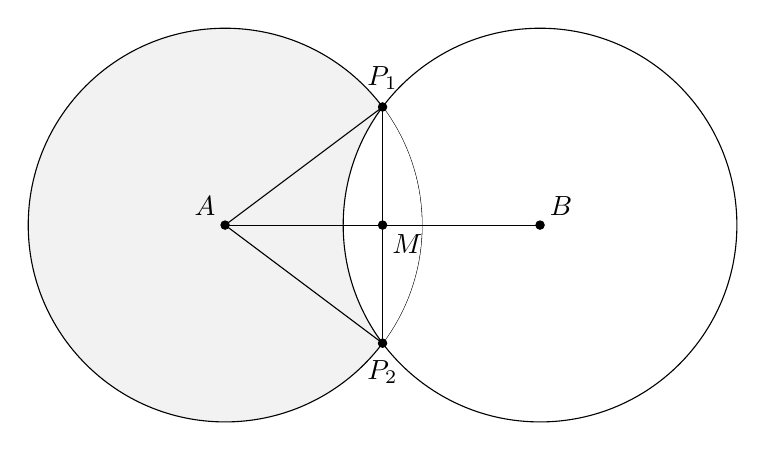
\begin{tikzpicture}[xscale=0.5,yscale=0.5]
    \filldraw[fill=black!5] (-4,0) circle (5);
    \scope
        \clip (-4,0) circle (5);
        \fill[white] (4,0) circle (5);
    \endscope
    \draw (4,0) circle (5);
    \filldraw (-4,0) circle[radius=3pt] node[above left] {$A$};
    \filldraw (4,0) circle[radius=3pt] node[above right] {$B$};
    \filldraw (0,3) circle[radius=3pt] node[above=1mm] {$P_1$};
    \filldraw (0,-3) circle[radius=3pt] node[below=1mm] {$P_2$};
    \filldraw (0,0) circle[radius=3pt] node[below right] {$M$};
    \draw (-4,0) -- (4,0);
    \draw (-4,0) -- (0,3);
    \draw (-4,0) -- (0,-3);
    \draw (0,-3) -- (0,3);
    \end{tikzpicture}
\end{figure}

There's a lot to discuss in this figure.  What we need to do is figure out how to find the area of the intersection and then subtract it from the area of the circle.  We redefine this as the area of the circle minus twice the segment cut off by $P_1P_2$ and its corresponding arc.  That area is equal to the area of the sector created between $P_1$, $A$, and $P_2$ and triangle $AP_1P_2$.

The area of circle $A$ is $\pi\left(4\sqrt{2}\right)^2=32\pi$.

Since $A$ is at $-4-4i$ and $B$ is at $4-4i$, we find that $$AB=||(4-4i)-(-4-4i)||=||8||=8.$$  Since $M$ is defined as the midpoint, $AM=4$.

We know that, because of the radius of $A$, $AP_1=4\sqrt{2}$.  Using the Pythagorean Theorem, we get $$P_1M=\sqrt{(4\sqrt{2})^2-(4)^2}=\sqrt{32-16}=4.$$

Since $AM=P_1M$, this means $\angle P_1AM=\angle AP_1M=45^{\circ}.$  We then reason that $\angle P_2AM=45^{\circ}$ as well since the triangles are congruent (SSS or SAS can prove this with ease).  Adding $\angle P_1AM$ and $\angle P_2AM$, we get $\angle P_1AP_2=90^{\circ}$.

Since $\angle P_1AP_2=90^{\circ}$, that means that the sector cuts off exactly one-quarter of the circle.  Thus, the area of the sector is $\dfrac{1}{4}(32\pi)=8\pi.$

The area of $\triangle P_1AP_2$ is $\dfrac{1}{2}(4)(8)=16$.  This means that the area between the segment $P_1P_2$ and arc $P_1P_2$ is $8\pi-16$.

To find the final area, we subtract twice this (since there are two of these in the intersection) from the area of the circle, which is $32\pi-2(8\pi-16)=\boxed{16\pi+32}.$ $\Box$\vspace{3mm}

\noindent \textbf{Challenge . 4}

(a) $\displaystyle \dfrac{1}{\overline{1/\overline{z}}}=\dfrac{1}{\dfrac{1}{z}}=\boxed{z}$. $\Box$

(b) Since $x=\dfrac{1}{\overline{z}}$, we reason that $z=\dfrac{1}{\overline{x}}$.  This gives $$\dfrac{1+i}{\overline{x}}-\dfrac{1-i}{x}=i \implies (1+i)x-(1-i)\overline{x}=ix\overline{x}.$$
Letting $x=a+bi$, we find that \begin{align*}
    (1+i)(a+bi)-(1-i)(a-bi)&=i(a+bi)(a-bi) \\
    (a-b)+(a+b)i-(a-b)-(-a-b)i&=i(a^2+b^2) \\
    2(a+b)i&=i(a^2+b^2) \\
    2(a+b)&=a^2+b^2 \\
    (a^2-2a)+(b^2-2b)&=0 \\
    (a-1)^2+(b-1)^2&=2
\end{align*}
If you don't know what happened in these last two steps, review the Completing the Square section in Chapter 5.  The final line shows that $x$ traces a $\boxed{\text{circle of radius } 2 \text{ with a center at } (1,1)}.$  $\Box$\vspace{3mm}

\noindent \textbf{Challenge . 5}

Note that we've seen the same denominator before when solving complex equations.  We've seen it two different places: when discussing the magnitude of $z$ and when discussing how to find $\dfrac{1}{z}$.  Since the magnitude of $z$ doesn't work nicely in solving equations, we'll discuss $1/z$ instead.

Let $z=x+yi$.  This means that $$\dfrac{1}{z}=\dfrac{1}{x+yi}=\dfrac{x-yi}{x^2+y^2}.$$  If we treat the first equation as the real component to a complex equation, and the second equation as the complex component, we get $$\left(x+\dfrac{x+8y}{x^2+y^2}\right)+\left(y+\dfrac{8x-y}{x^2+y^2}\right)i=2+0i.$$ Doing some rearranging, we get $$x+yi+\dfrac{x-yi}{x^2+y^2}+\dfrac{8(y+xi)}{x^2+y^2}=2 \implies z+\dfrac{1}{z}+\dfrac{8(y+xi)}{x^2+y^2}=2.$$
Now we need a way to express the third term in terms of $z$.  We know that $y+xi=i(x-yi)$, so we get $$z+\dfrac{1}{z}+\dfrac{8i}{z}=2.$$  All we need to do is solve for $z$.  Multiplying $z$ on both sides, we get $z^2+1+8i=2z$.  Rearranging, we get $z^2-2z+1=-8i$, which means that $(z-1)^2=-8i$.  We assign complex number $w=z-1$ to make this easier.  We are now looking for $w$ such that $w^2=-8i$.

Let $w=\alpha+\beta i$.  Thus, $\alpha^2-\beta^2+2\alpha\beta=-8i.$  This means that $\alpha^2-\beta^2=0$ an $\alpha\beta=-4$.  Simplifying the first, we get $\alpha=-\beta$ (because the product must be negative).  This means that either $\alpha=-\beta=-2$ or $\alpha=-\beta=2$.  Finding both solutions, we get $z-1=-2+2i$ and $z-1=2-2i$.  This means we have the solutions $z_1=-1+2i$ and $z_2=3-2i$.  These correspond with the ordered pairs $\boxed{(-1,2) \text{ and } (3,-2)}$. $\Box$\vspace{3mm}

\noindent \textbf{Challenge . 6}

We know that a number is real if $z=\overline{z}$.  Using the magnitude parameter, we know that $||z_1||=1$, which means that $z_1\overline{z_1}=1 \implies \overline{z_1}=\dfrac{1}{z_1}$.  Likewise, $\overline{z_2}=\dfrac{1}{z_2}$. Computing the conjugate, we get $$\overline{z}=\overline{\dfrac{4z_1z_2}{\left(z_1+z_2\right)^2}}=\dfrac{4\overline{z_1}\overline{z_2}}{(\overline{z_1}+\overline{z_2})^2}=\dfrac{4\dfrac{1}{z_1}\dfrac{1}{z_2}}{\left(\dfrac{1}{z_1}+\dfrac{1}{z_2}\right)^2}=\dfrac{4\dfrac{1}{z_1}\dfrac{1}{z_2}(z_1+z_2)^2}{(z_1+z_2)^2}=\dfrac{4z_1z_2}{\left(z_1+z_2\right)^2}=\boxed{z}.$$

We know that a number is imaginary if $z=-\overline{z}$.  Using the same condition $z_1\overline{z_1}=1 \implies \overline{z_1}=\dfrac{1}{z_1}$ and $\overline{z_2}=\dfrac{1}{z_2}$.  Plugging into the imaginary condition, we get $$\overline{z}=\overline{\dfrac{z_1+z_2}{z_1-z_2}}=\overline{\dfrac{z_1+z_2}{z_1-z_2}}=\dfrac{\dfrac{1}{z_1}+\dfrac{1}{z_2}}{\dfrac{1}{z_1}-\dfrac{1}{z_2}}=\dfrac{z_1+z_2}{z_2-z_2}=-\left(\dfrac{z_1+z_2}{z_1-z_2}\right)=\boxed{-z}.$$ $\Box$

%%%%%%%%%%%%%%%%%%%%%%%%%%%%%% CHAPTER 4 %%%%%%%%%%%%%%%%%%%%%%%%%%%%%%%%%%%%%%%%%%%%%
\chapter{Linear Functions and Relations}

\noindent \textbf{Review . 1}

All of these problems intend to demonstrate mastery of the definition of an inverse.  Remember that the inverse is a reflection of the graph over the line $y(x)=x$.  There's not much explanation to be given here; we just need to know how to determine the shape of the reflection.

(a) \begin{figure}[!ht]
    \centering
    \begin{tikzpicture}[xscale=0.20,yscale=0.20]
      \draw[<->] (-10,0) -- (10,0) node[right] {$x$};
      \draw[<->] (0,-10) -- (0,10) node[above] {$y(x)$};
      \draw[scale=1,samples=100,domain=-10:10,variable=\x,black,dashdotted] plot({\x},{\x});
      \draw[scale=1,samples=100,domain=-10:10,variable=\x,black] plot({\x},{4}) node[right] {$f(x)$};
      \draw[scale=1,samples=100,domain=-10:10,variable=\y,black] plot({4},{\y}) node[right] {$f^{-1}(x)$};
    \end{tikzpicture}   
\end{figure} $\Box$\vspace{3mm}

(b) \begin{figure}[!ht]
    \centering
    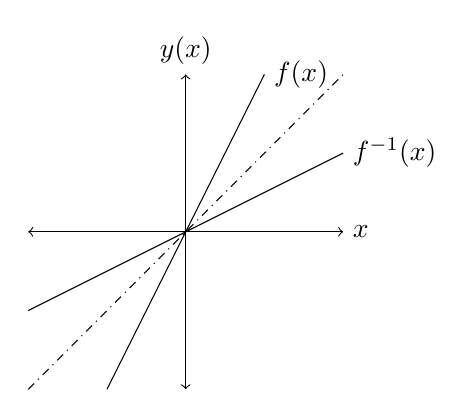
\begin{tikzpicture}[xscale=0.20,yscale=0.20]
      \draw[<->] (-10,0) -- (10,0) node[right] {$x$};
      \draw[<->] (0,-10) -- (0,10) node[above] {$y(x)$};
      \draw[scale=1,samples=100,domain=-10:10,variable=\x,black,dashdotted] plot({\x},{\x});
      \draw[scale=1,samples=100,domain=-5:5,variable=\x,black] plot({\x},{2*\x}) node[right] {$f(x)$};
      \draw[scale=1,samples=100,domain=-5:5,variable=\y,black] plot({2*\y},{\y}) node[right] {$f^{-1}(x)$};
    \end{tikzpicture}   
\end{figure} $\Box$\vspace{3mm}

(c) \begin{figure}[!ht]
    \centering
    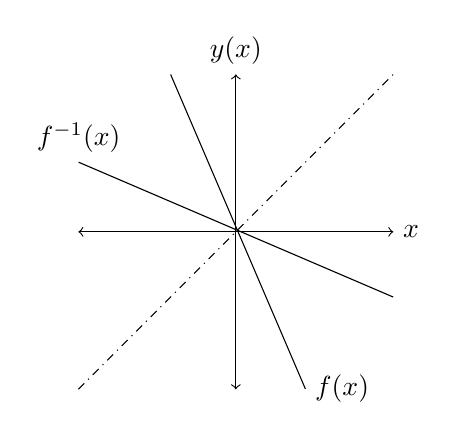
\begin{tikzpicture}[xscale=0.20,yscale=0.20]
      \draw[<->] (-10,0) -- (10,0) node[right] {$x$};
      \draw[<->] (0,-10) -- (0,10) node[above] {$y(x)$};
      \draw[scale=1,samples=100,domain=-10:10,variable=\x,black,dashdotted] plot({\x},{\x});
      \draw[scale=1,samples=100,domain=-4.14:4.42,variable=\x,black] plot({\x},{(1-7*\x)/3}) node[right] {$f(x)$};
      \draw[scale=1,samples=100,domain=-4.14:4.42,variable=\y,black] plot({(1-7*\y)/3},{\y}) node[above] {$f^{-1}(x)$};
    \end{tikzpicture}   
\end{figure} $\Box$\vspace{3mm}
\newpage
(d) \begin{figure}[!ht]
    \centering
    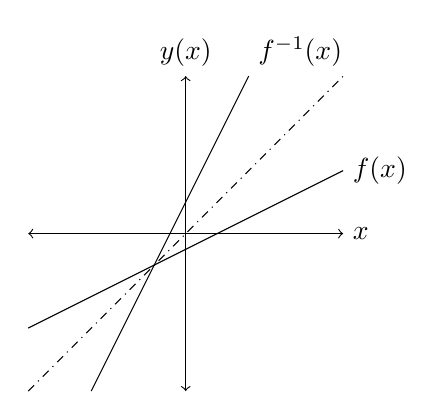
\begin{tikzpicture}[xscale=0.20,yscale=0.20]
      \draw[<->] (-10,0) -- (10,0) node[right] {$x$};
      \draw[<->] (0,-10) -- (0,10) node[above] {$y(x)$};
      \draw[scale=1,samples=100,domain=-10:10,variable=\x,black,dashdotted] plot({\x},{\x});
      \draw[scale=1,samples=100,domain=-10:10,variable=\x,black] plot({\x},{\x/2-1}) node[right] {$f(x)$};
      \draw[scale=1,samples=100,domain=-10:10,variable=\y,black] plot({\y/2-1},{\y}) node[above right] {$f^{-1}(x)$};
    \end{tikzpicture}   
\end{figure} $\Box$\vspace{3mm}

\noindent \textbf{Review . 2}

There is honestly no trick to this question.  Simply combine the fractions and solve for $x$.  $$x-\dfrac{3}{4}=\dfrac{1}{12} \implies x=\dfrac{3}{4}+\dfrac{1}{12}=\boxed{\dfrac{5}{6}}.$$ $\Box$\vspace{3mm}

\noindent \textbf{Review . 3}

Again, for this question, we just need to ensure that we graph each part in their respective locations.  We know how to graph each function; consider each domain by finding the endpoints for each section. \begin{align*}
    y_1(x) &: y_1(-\infty)=-\infty \hspace{0.25in} y_1(2)=1 \\
    y_2(x) &: y_2(2)=-6 \hspace{0.51in} y_2(3)=-\dfrac{19}{2} \\
    y_3(x) &: y_3(3)=4 \hspace{0.62in} y_3(\infty)=4
\end{align*}
Be sure to recognize whether the endpoints are inclusive or exclusive for each section.
\begin{figure}[!ht]
    \centering
    \begin{tikzpicture}[xscale=0.25,yscale=0.25]
      \draw[<->] (-10,0) -- (10,0) node[right] {$x$};
      \draw[<->] (0,-10) -- (0,10) node[above] {$y(x)$};
      \draw[scale=1,samples=100,domain=-3.5:2,variable=\x,black] plot({\x},{2*\x-3});
      \draw[scale=1,samples=100,domain=2:3,variable=\x,black] plot({\x},{1-7*\x/2});
      \draw[scale=1,samples=100,domain=3:10,variable=\x,black] plot({\x},{4});
      \filldraw (2,1) circle[radius=7pt];
      \filldraw (3,-9.5) circle[radius=7pt];
      \draw (2,-6) circle[radius=7pt];
      \draw (3,4) circle[radius=7pt];
    \end{tikzpicture}   
\end{figure} $\Box$\vspace{3mm}

\noindent \textbf{Review . 4}

This problem was a bit of a trick question.  In all cases, the domain is $\mathbb{R}$ because they are polynomial functions.  Since they are linear functions, the range is also $\mathbb{R}$.  So, we will write the domain and range as $\boxed{\begin{matrix} x\in\mathbb{R} \\ y\in\mathbb{R}\end{matrix}}$. $\Box$

\noindent \textbf{Review . 5}

Again, just like \textbf{Review . 2}, we just have to solve this for $x$, but this time it's a bit more complicated.  Once we combine some of the stacked fractions, we will have a much easier problem.  $$x-\dfrac{1}{4}-\dfrac{3x}{8}=\dfrac{2}{3}-\dfrac{x}{8}-\dfrac{11}{12} \implies \dfrac{5x}{8}-\dfrac{1}{4}=-\dfrac{x}{8}-\dfrac{1}{4} \implies \boxed{x=0}.$$ 
Make sure you see how we quickly jumped to that conclusion.  Since the constants are equal, we know that the variable terms must equal, which is only true when $x=0$.  $\Box$\vspace{3mm}

\noindent \textbf{Review . 6}

For each of these problems, we will write the given word problem as a numeric equation and solve for the value needed.

(a) $\displaystyle x=7x-18 \implies -6x=-18 \implies \boxed{x=3}.$ $\Box$\vspace{3mm}

(b) $\displaystyle x=4x-75 \implies -3x=-75 \implies \boxed{x=25}.$ $\Box$\vspace{3mm}

(c) $\displaystyle 2x-12=3x-15 \implies -x=-3 \implies \boxed{x=3}.$ $\Box$\vspace{3mm}

(d) $\displaystyle 2x-5=x+18 \implies \boxed{x=23}.$ $\Box$\vspace{3mm}

\noindent \textbf{Review . 7}

We seek the smallest integer value of $n$ such that $f(n)>0$.  So, we plug in this inequality and solve for $n$.  $$\dfrac{4n-5}{12}>0 \implies 4n-5>0 \implies n>\dfrac{5}{4}.$$  The smallest integer in this interval is $\boxed{n=2}.$ $\Box$ \vspace{3mm}

\noindent \textbf{Review . 8}

The intersection point must always be on the line $y(x)=x$, so we can make this substitution.  $$x=\dfrac{1}{3}x-3 \implies \dfrac{2}{3}x=-3 \implies \boxed{x=-2}.$$ $\Box$\vspace{3mm}

\noindent \textbf{Review . 9}

(a) $x=f^{-1}(x)-1 \implies f^{-1}(x)=\boxed{x+1}.$ $\Box$\vspace{3mm}

(b) $x=\dfrac{2f^{-1}(x)-1}{3} \implies 3x=2f^{-1}(x)-1\implies f^{-1}(x)=\boxed{\dfrac{3x+1}{2}}.$ $\Box$\vspace{3mm}

(c) $x=\dfrac{5}{6}f^{-1}(x)-\dfrac{4}{5}\implies x+\dfrac{4}{5}=\dfrac{5}{6}f^{-1}(x) \implies f^{-1}(x)=\boxed{\dfrac{6}{5}x+\dfrac{24}{25}}.$ $\Box$\vspace{3mm}

(d) $x=a_1f^{-1}(x)+a_2 \implies x-a_2=a_1f^{-1}(x)\implies f^{-1}(x)=\boxed{\dfrac{1}{a_1}x-\dfrac{a_2}{a_1}}.$ $\Box$\vspace{3mm}

\noindent \textbf{Review . 10}

As seen in part D of the previous example, if $a_1=a_2=k$, the inverse of the function is $f^{-1}(x)=\dfrac{1}{k}x-1.$  Multiplying this by $f(x)=kx+k$, we get $$\left(kx+k\right)\left(\dfrac{1}{k}x-1\right)=x^2+\left(1\right)x-(k)x-k=x^2+(1-k)x-k.$$
To make this equal to $x^2-3x-4$, by inspection, we know that $\boxed{k=4}$. $\Box$\vspace{3mm}

\noindent \textbf{Review . 11}

Using the basic information provided, we deduce the equation $F=k\cdot \Delta x$.  This is known as \textit{Hooke's Law}.  To find the spring constant, we just need to use one of the values in the equation.  We'll use the first one, but it really doesn't matter.  $$1.5\text{ N}=k(0.25\text{ m}) \implies \boxed{k=6 \text{ N}/\text{m}}.$$ $\Box$\vspace{3mm}

\noindent \textbf{Review . 12}

For this question, we need to find the value of $k$ such that $f_1(k)=f_2(k).$  $$1-2k=\dfrac{3}{2}k-5 \implies -\dfrac{7}{2}k=-6 \implies \boxed{k=\dfrac{12}{7}}.$$ $\Box$\vspace{3mm}

\noindent \textbf{Review . 13}

We can see that the first equation given almost represents slope; it's simply missing the denominator.  If we put the denominator in there, we get $$\dfrac{f(6)-f(2)}{6-2}=\dfrac{12}{4}=3.$$  This means that the slope is $48$.  Using this to manipulate the goal, we get $$\dfrac{f(12)-f(2)}{12-2}=3 \implies f(12)-f(2)=\boxed{30}.$$ $\Box$\vspace{3mm}

\noindent \textbf{Review . 14}

Graphing gives us the best idea to what this is.  

\begin{figure}[!ht]
    \centering
    \begin{tikzpicture}[xscale=0.50,yscale=0.50]
      \draw[<->] (-3,0) -- (3,0) node[right] {$x$};
      \draw[<->] (0,-3) -- (0,3) node[above] {$y(x)$};
      \draw[scale=1,samples=100,domain=-1:2,variable=\x,black] plot({\x},{1-2*\x});
    \end{tikzpicture}   
\end{figure}

The area that we need to find is the area between the axes and the graph, which is a right triangle.  To find the area, we can find the intercepts to determine the lengths of the legs.  When $f(x)=0$, $x=\dfrac{1}{2}$, and then $x=0$, $f(0)=1$.  Finding the area, we get $$A=\dfrac{1}{2}bh=\dfrac{1}{2}\left(1\right)\left(\dfrac{1}{2}\right)=\boxed{\dfrac{1}{4}}.$$ $\Box$\vspace{3mm}
%%%%%%%%%%%%%%%%%%%%%%%%%%%%%% CHAPTER 5 %%%%%%%%%%%%%%%%%%%%%%%%%%%%%%%%%%%%%%%%%%%%%
\chapter{Quadratic Functions}

%%%%%%%%%%%%%%%%%%%%%%%%%%%%%% CHAPTER 6 %%%%%%%%%%%%%%%%%%%%%%%%%%%%%%%%%%%%%%%%%%%%%
\chapter{Higher-Order Polynomials}

%%%%%%%%%%%%%%%%%%%%%%%%%%%%%% CHAPTER 7 %%%%%%%%%%%%%%%%%%%%%%%%%%%%%%%%%%%%%%%%%%%%%
\chapter{Rational Functions}

%%%%%%%%%%%%%%%%%%%%%%%%%%%%%% CHAPTER 8 %%%%%%%%%%%%%%%%%%%%%%%%%%%%%%%%%%%%%%%%%%%%%
\chapter{Radicals and Rational Exponents}

%%%%%%%%%%%%%%%%%%%%%%%%%%%%%% CHAPTER 9 %%%%%%%%%%%%%%%%%%%%%%%%%%%%%%%%%%%%%%%%%%%%%
\chapter{Exponential and Logarithmic Functions}

%%%%%%%%%%%%%%%%%%%%%%%%%%%%%% CHAPTER 10 %%%%%%%%%%%%%%%%%%%%%%%%%%%%%%%%%%%%%%%%%%%%%
\chapter{Further Piece-wise Functions}

%%%%%%%%%%%%%%%%%%%%%%%%%%%%%% CHAPTER 11 %%%%%%%%%%%%%%%%%%%%%%%%%%%%%%%%%%%%%%%%%%%%%
\chapter{Essentials for Physics}

%%%%%%%%%%%%%%%%%%%%%%%%%%%%%% CHAPTER 12 %%%%%%%%%%%%%%%%%%%%%%%%%%%%%%%%%%%%%%%%%%%%%
\chapter{Systems of Equations}

%%%%%%%%%%%%%%%%%%%%%%%%%%%%%% CHAPTER 13 %%%%%%%%%%%%%%%%%%%%%%%%%%%%%%%%%%%%%%%%%%%%%
\chapter{Trigonometry}

%%%%%%%%%%%%%%%%%%%%%%%%%%%%%% CHAPTER 14 %%%%%%%%%%%%%%%%%%%%%%%%%%%%%%%%%%%%%%%%%%%%%
\chapter{Conic Sections}

%%%%%%%%%%%%%%%%%%%%%%%%%%%%%% CHAPTER 15 %%%%%%%%%%%%%%%%%%%%%%%%%%%%%%%%%%%%%%%%%%%%%
\chapter{Inequalities}

%%%%%%%%%%%%%%%%%%%%%%%%%%%%%% CHAPTER 16 %%%%%%%%%%%%%%%%%%%%%%%%%%%%%%%%%%%%%%%%%%%%%
\chapter{Advanced Problem-Solving}
\end{document}